\documentclass[20pt]{article}
\usepackage{graphicx}
\setlength\parindent{0pt}
\usepackage{amsfonts}
\usepackage{courier}
\begin{document}
\title{Soundcool's Player Specification}
\maketitle

This is a specification for soundcool's player module.
\section*{User interface}
Following is the user interface for an player module in Soundcool:

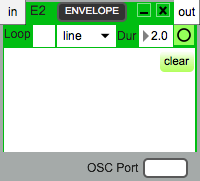
\includegraphics[scale=0.5]{gui.png} 

\begin{itemize}
 \item \textbf{Speed, Volume, Loop, Reverse} Each independent controls that are same definition as named.  \textbf{They are fixed parameter in player module, which means that they don't change with the selection of audio. Other parameters (play/pause, stop, progress bar, time) will be reset after a switch of audio.} 
    \item \textbf{Audio Progress Bar:} User can drag to change progress. This is disabled until actual audio is being selected. \\
    When Reverse is \textit{True}, the Audio Progress is left-right mirrored. Note that this means when audio finished playing backward, the progress bar will jump back to rightmost, the "starting point"
    \item \textbf{Time:} Denoting the progression time of the audio. Notice that it doesn't denote actual time, but more of sample rate, so this 'time' will go faster at higher speed.
    \item \textbf{Play/Pause:} After clicking play the play button will become pause button. this is a parameter that will get reset as a change of audio. 
    \item   \textbf{Stop}: When reverse is \textit{False} Clicking stop will result in audio progress back to 0. When the audio is reversed playing the Stop will goes back to rightmost. 
    \item \textbf{Open audio:} There will be a list of audio for your selection. Note that progress bar, play/pause and time will be reset after a new audio get selected. Note that \textit{reverse} is not going to be reset, so if reverse is \textit{true}, the new audio will start with rightmost progress bar and max time. \\
    (optional) In web audio soundcool, there should be an option of uploading audio in the player module, so that user doesn't need to go back to soundpage to upload sound.
\end{itemize}

\section*{Web Audio Implementation}

\subsection*{Attributes}
\subsubsection*{\texttt{buffer:Float32Array}} 
A \texttt{Float32Array} containing discrete audio samples.

\subsubsection*{\texttt{startTime:number}}
Attribute indicating when playback started. \texttt{null} if audio isn't played. 

\texttt{AudioContext.currentTime} is used to set the value of this attributes.

\subsubsection*{\texttt{offset:number}}
This attribute is used to store the state of playhead (in seconds) for stateful operations like \texttt{pause} and \texttt{seek}, so \texttt{play} knows where to start playing from.

\subsection*{Methods}
\subsubsection*{\texttt{load(url)}}
This method makes a \texttt{XMLHttpRequest} and loads decoded samples into a \texttt{Float32Array} buffer. Input argument \texttt{url} is the URL of the audio to be loaded. Returns a \texttt{Promise} object which when resolved returns the length of the audio in seconds. The pending promise will be rejected upon failure to load the audio.

\subsubsection*{\texttt{play()}}
This method instantiates a Web Audio \texttt{AudioBufferSourceNode(ABSN)} and starts playback from \texttt{offset} seconds. It will internally apply player properties like \texttt{loop} and \texttt{playbackRate} that were previously set or saved.

\subsubsection*{\texttt{stop(resetOffset=true)}}
Method to stop the playback. \texttt{resetOffset}, a \texttt{boolean}, specifies if \texttt{offset} should reset to 0.

\subsubsection*{\texttt{pause()}}
This method will pause the playback that can be resumed by calling \texttt{play} method.

\subsubsection*{\texttt{reverse()}}
A method to reverse the playback of the audio. The implementation reverses the \texttt{buffer}, re-instantiate \texttt{ABSN} and resumes playback from reversed \texttt{offset}.

\subsubsection*{\texttt{seek(seekPosition)}}
This method is used to jump to a certain duration and continue playback from that point onwards. \texttt{seekPosition}, a \texttt{number} in the range [0, 1], specifies what fraction of audio to skip. For example, 
\begin{itemize}
\item \texttt{seekPosition} of 0.0 will start playback from the start of the audio.
\item \texttt{seekPosition} of 0.5 will start playback from the middle of the audio.
\item \texttt{seekPosition} of 1.0 will start playback from the end of the audio.
\end{itemize}

Note: \texttt{seekPosition} is independent of playback \texttt{speed} and/or if the buffer is \texttt{reversed}.

\subsubsection*{\texttt{set speed:number}}
This setter will set the playback speed of the player. Speed value is a non-negative float \texttt{number}. 
\begin{itemize}
\item \texttt{speed} of 1.0 plays the audio at full speed, or 44,100 Hz.
\item \texttt{speed} of 0.5 plays the audio at half speed, or 22,050 Hz.
\item \texttt{speed} of 2.0 doubles the audio's playback rate to 88,200 Hz.
\end{itemize}

\subsubsection*{\texttt{set loop:boolean}}
Set \texttt{loop} to \texttt{true} for audio to repeat indefinitely from start after full audio playback.

\section*{Implementation Notes}
\begin{itemize}
\item Disable operations \texttt{play}, \texttt{pause}, \texttt{seek} and \texttt{reverse} when there is no loaded audio.
\end{itemize}
\end{document}